\documentclass{article}

\usepackage[numbers]{natbib}
\usepackage{hyperref}
\usepackage{xcolor}
\hypersetup{
  colorlinks,
  linkcolor={red!50!black},
  citecolor={blue!50!black},
  urlcolor={blue!80!black}
}
\usepackage{algorithm}
\usepackage{amsfonts}
\usepackage{amsmath}
\newtheorem{definition}{Definition}
\usepackage{algpseudocode}
\usepackage{graphicx}
\usepackage{enumitem}
\usepackage{pgfplots}
\pgfplotsset{width=6cm,compat=1.9}

\algrenewcommand\algorithmicrequire{\textbf{Input:}}
\algrenewcommand\algorithmicensure{\textbf{Output:}}
\usepackage{xcolor}

\title{\texttt{dpsa4fl}: Differential Privacy \\ for \\ Federated Machine
  Learning \\ with Prio}
\author{Olivia Roehrig  \\
	\and
	Maxim Urschumzew \\
	\textit{Determi} \\
	}

\date{\today}
% Hint: \title{what ever}, \author{who care} and \date{when ever} could stand 
% before or after the \begin{document} command 
% BUT the \maketitle command MUST come AFTER the \begin{document} command! 
\begin{document}

\maketitle


\begin{abstract}
We present \texttt{dpsa4fl}, a framework for differentially private federated
learning with secure aggregation using the prio protocol. It enables training a
neural network in a decentralized setting with differential privacy for data
owners without disclosing sensitive data to any protocol participant or
requiring trust in a single server. Given an appropriate threat model, it also
provides resistance to malicious clients attempting data poisoning attacks by
leveraging distributed input validation.
\end{abstract}

\section{Introduction}
Data privacy is one of the factors motivating \emph{federated learning} (FL). A
machine learning model can be trained locally on computers owned by data owners
(\emph{clients}), who exchange only intermediate training results
(\emph{gradients}), instead of the data itself, with a central server that
aggregates them into a shared model~\cite{McMahan2016CommunicationEfficientLO}.
While this relieves the need to collect possibly sensitive data in a central
location to perform the training, the shared model and the gradients themselves
contain enough information to enable reconstruction of private
information~\cite{7958568,Boenisch2021WhenTC}.

A solution to this problem is using a modified training algorithm that provides
\emph{differential privacy} (DP) for the model~\cite{Abadi_2016}. The technique adds
a small amount of noise to the result of each training step, calibrated in a way
that makes high certainty statements about the presence of an individual point
in the training dataset unlikely to be inferable from the model.

Adding noise locally would require a large amount of noise and hence large
utility loss to achieve privacy, while globally adding noise after the training
step would require some party to have access to the non-noised aggregate.

\emph{Secure aggregation} (SA) is a technique for multiple
participants to compute a function on their confidential data that reveals only
the computation result without disclosing any other information about the
inputs to anyone. This can be leveraged to enable adding the noise after aggregating
intermediate results, but keep the individual contributions and the non-noised
aggregate secret (\emph{Server-DP}~\cite{dprio}).

\paragraph{Contributions.}
We present \texttt{dpsa4fl}, a system which provides Server-DP with
secure aggregation for federated learning. Our privacy guarantees cover the training
result, as well as all intermediate aggregation and computation steps. We employ the
prio protocol~\cite{prio} for secure aggregation.

We implement \texttt{dpsa4fl} as a set of wrapping layers which make prio usable
from federated learning pipelines. In order for
them to be usable for machine learning, we have to add support for gradient
vector types, in particular with a verified L2-norm bound. We use
\texttt{flower}~\cite{flower} as our target federated learning framework.
Concretely, we did the following:
\begin{itemize}
  \setlength\itemsep{0em}
\item We designed a ``prio type'' for aggregation of gradient vectors with
  bounded L2-norm for \texttt{libprio-rs}~\cite{libprio-rs}, a rust implementation
  of the prio protocol.
\item We added functionality for server differential privacy in
  \texttt{libprio-rs} and \texttt{janus}~\cite{janus}, a rust implementation of
  the server infrastructure required for Prio.
\item We developed supporting infrastructure for integrating \texttt{janus} into
  a federated learning pipeline.
\item We built bindings to use our system from the \texttt{flower} federated
  learning framework.
\end{itemize}
All code is available as open source, see the respective repositories\footnotemark{} for more
documentation. In this paper we present the overall architecture as well as a
privacy and utility analysis.

\footnotetext{The core library is \texttt{dpsa4fl}~\cite{dpsa4fl}.\newline
  \hspace*{1.8em}Python bindings are provided in
  \texttt{dpsa4fl-bindings.py}~\cite{dpsa4fl-bindings}.\newline
  \hspace*{1.8em}The integration with \texttt{flower} is \texttt{dpsa4flower}~\cite{dpsa4flower}.
}

\paragraph{Privacy and correctness guarantees.}
Our system requires two aggregation servers that do not collude with each other or clients, one of which must honestly follow protocol. All other participants, namely the clients and a server coordinating federated model updates, can be malicious. We assume that a client interested in their own data's differential privacy executes the protocol correctly. In this setting, we can guarantee anonymity (no adversary can tell which client submitted which data value) and privacy (no adversary learns anything about any honest clients' data values except the differentially private aggregate) as well as differential privacy for all information exchanged about an honest client between all participants as well as the final training result.

If we can assure both aggregation servers to honestly follow protocol, even while curious, our system is robust towards data poisoning attacks by ensuring differential privacy even for malicious clients and hence limiting the influence any single client can have on the aggregation result.

\paragraph{Related work.}
There is a variety of existing work centered around subsets of
$\{\textrm{DP}, \textrm{FL}, \textrm{SA}, \textrm{SA with input validation}\}$ with varying
architectures and threat models. The most closely related is
DPrio~\cite{dprio} by Keeler et al.,\ who propose a different mechanism for
adding differential privacy to the prio protocol. They thus have a very similar
threat model and input validation capabilities as our approach. A substantial
difference is that in their protocol, the noise to be added for differential
privacy is generated by the clients, and the aggregation servers are merely
tasked with selecting a subset of clients whose noise they include in the
aggregate. This means that their privacy guarantee depends on the fraction of
honest clients, while our guarantee only requires one out of two aggregators to
be honest.

{\color{green}TODO: add missing references}
There is a series of papers~\cite{Kairouz2021TheDD}~\cite{}~\cite{} based on the original
SecAgg~\cite{secagg} protocol by Bonawitz et al. They follow the explicit goal
of providing differential privacy specifically for FL tasks. SecAgg is a protocol
with a single-server architecture, which means that the threat model, and thus
the trade-offs in protocol design, are quite different from the ones used in the present work.
Additionally, SecAg currently does not integrate input validation and hence does not protect
against malicious clients.

{\color{green}TODO: add missing references}
Approaches to secure aggregation with input validation other than prio are based on
\textit{ring learning with errors}, such as RoFL~\cite{rofl} and ACORN~\cite{acorn}.
While in RoFL, the input validation results in an 48x increase in communication
costs, ACORN is successful in reducing the overhead to 2--10x. Unfortunately,
with these being single-server architectures as well, it is not immediately
clear how differential privacy could be added in a way that the aggregator
server does not see the non-noised sum of gradients. Protection against inference
attacks such as~\cite{7958568} hence can only be guaranteed if the server is honest.

An approach which integrates differential privacy but not input validation
is FLDP~\cite{Stevens2021EfficientDP} by Stevens et al. They achieve an overhead
of 1.7x.

{\color{green}TODO: add missing reference, also in footnote}
Finally, with all mentioned work being mostly theoretical papers, the
options for actually running real-world FL tasks seem to be few:
\begin{itemize}
  \setlength\itemsep{0em}
\item There are building blocks for both secure aggregation (based on SecAgg) and for local or
  global differential privacy in flower\footnote{See the documentation here~\cite{} and
    here~\cite{}}, but simply putting them together does not protect against inference
  attacks.{\color{green}TODO: why?}
\item The authors of DPrio provide source code~\cite{} for their empirical evaluation in
  terms of a simulation of FL, but such simulation code is far from enough for
  real-world deployments.
\item In a similar vein, the authors of e.g.~\cite{Kairouz2021TheDD} provide
  source code which is based on TensorFlow Federated~\cite{tff}. Unfortunately this
  framework is currently only usable for simulations as well.
\end{itemize}



\section{Preliminaries}

\subsection{Federated Learning}
Federated learning is a machine learning technique introduced
by~\citet{FL}, aiming to avoid centralized data collection by a single
party performing the training. Instead, clients obtain a copy of
the global model and train it on their private data locally. Model updates are
then collected by a central party (\emph{FL~server}) and aggregated into an update for
the global model. The updated global model is distributed to the clients again and the
procedure is repeated until model performance is satisfactory.

While removing the need for central data collection, the above scheme still
requires clients to disclose the model updates they derived from their private
data, which contain enough information for reconstruction attacks like the ones
detailed in~\cite{7958568,Boenisch2021WhenTC}. It seems that differential
privacy combined with secure aggregation is the best approach to
preserve the clients' privacy in this setting. See~\cite{fl-survey} for an extensive survey.

\subsection{Secure Aggregation and Input Validation}
Secure aggregation allows for the aggregation of secret distributed data in a
way that reveals only the aggregate result. More concretely, let
$x_1,\ldots,x_n$ be private values, each located at one of $n$ clients. The goal of SA
is to compute a given function $f(x_1,\ldots,x_n)$ in a way that every
participant learns at most as much about the input values $x_1,\ldots,x_n$
as can be deduced mathematically from only knowing the result of $f$.

{\color{red}TODO: add reference}

A topic related to SA is input validation. In some cases, it might be
required that the data submitted by clients fulfills certain properties, such as
lying within certain numerical bounds. Since the aggregating servers
do not see the submissions in plaintext, they cannot easily check whether this
is the case. Solutions usually involve zero-knowledge proof
protocols, where aggregation servers or clients interact with each other in
order to convince themselves of the validity of the data---without revealing it.


\subsection{Differential Privacy}
Differential privacy is a method of enabling the publication of information derived from a dataset while making it unlikely that information about individual entries of the dataset can be inferred. There are many flavours of differential privacy, most of which can be converted into one another. A good introduction for programmers can be found here~\cite{near_abuah_2021}.

We define the variant we will be using throughout the paper, following~\cite{DBLP:journals/corr/BunS16}.
\begin{definition}[Zero-concentrated Differential Privacy]
A randomized function $M: \mathcal X\rightarrow Y$ is $\rho$-zero-concentrated differentially private if for all $X,X'\in \mathcal X$ differing in a single entry and all $\alpha\in(1,\infty)$,
$$D_\alpha(M(X)\|M(X'))\leq \rho\cdot\alpha$$
where $D_\alpha(M(X)\|M(X'))$ is the $\alpha$-Renyi divergence between the distributions of $M(X)$ and $M(X')$.
\end{definition}

The Renyi divergence is a way of measuring dissimilarity between distributions. Intuitively, the output distributions of a $\rho$-zero-concentrated differentially private function given two input datasets that differ in one entry will be harder to tell apart the smaller $\rho$. This means that one is unlikely to be able to tell whether an individual entry was an element of the input dataset when observing only the outputs of $M$.

One way of achieving differential privacy for a deterministic function $f$ is by adding noise drawn from a specific distribution calibrated to the \textit{sensitivity} 
$$\Delta f=\max\{\|f(X)-f(X')\|_2\}$$
of the function, where the maximum is taken over all datasets $X,X'$ differing in a single entry. For example, for an integer-valued function $f:\mathcal X\rightarrow \mathbb Z$ the randomized function
$$M(X) = f(X) + n \textnormal{ where } n \sim \mathcal N_\mathbb{Z}\left(0,\frac{(\Delta f)^2}{2\rho}\right)$$
is $\rho$-zero-concentrated differentially private~\cite[Proposition 1.6]{DBLP:journals/corr/abs-2004-00010}, where $\mathcal N_\mathbb{Z}(\mu, \sigma^2)$ denotes the discrete Gaussian distribution~\cite{DBLP:journals/corr/abs-2004-00010}.

\paragraph{Local vs.\ global differential privacy} In a distributed setting, it is relevant to consider at what point in the protocol the noise gets added.

Adding noise client-side (\textit{local} differential privacy) does not require entrusting a central party with the non-noised information and the correct execution of the noising. However, each client needs to add the amount of noise required for their privacy guarantee, while it would be sufficient to add that amount once to the sum of all gradients after aggregation.

The usual relief for this is adding noise on a central server (\textit{global} differential privacy). This requires trust in the noising party, as they get access to the non-noised aggregate and need to do the noising faithfully.

Another approach, which becomes viable in conjunction with some forms of secure aggregation, is
to perform noising on the aggregation servers prior to performing their computation on the encrypted
client inputs, so even the aggregators never see the non-noised aggregate gradient (this
technique has been coined Server DP~\cite{dprio}).

It is still more noise added than necessary in order to distribute the trust:
each server adds the full amount of noise necessary for all clients' guarantees,
allowing for all but one aggregator to maliciously deviate from protocol without
compromising differential privacy. However, with Server DP the noise scales with the number of
aggregation servers (of which only two are required, if the threat model allows it), while
with local DP it scales with the number of clients.

\paragraph{Robustness}

Differential privacy not only protects from inference attacks, but also limits the influence a single gradients' value can have on the training result. This is a viable defense against \textit{data poisoning attacks} by malicious clients attempting to sabotage or sway training results in their favour. Note that providing differential privacy for clients that don't have an interest in having differential privacy is not trivial in a setting where secure aggregation is used. A usual approach to bounding the sensitivity of many functions is bounding the inputs -- something that the noising parties cannot easily do if they don't have access to the plaintext values. Input validation is a relief, but in our case comes with additional trust requirements.

{\color{red}TODO: add reference}



\section{Secure aggregation with Prio}
The Prio protocol has been designed by Corrigan-Gibbs and Boneh in~\cite{prio} as a
way to securely aggregate client data with two aggregation servers. As long as
one server remains honest, the data remains private. One outstanding feature of
prio is that the validity of the submitted data can be verified by the
aggregators without them having access to the data itself (\textit{input
  validation}). This however requires \emph{both} servers to be honest.

The original prio protocol has since been improved, and, under the name of Prio3, integrated into the
more general framework of \textit{verifiable distributed aggregation
  functions}~\cite{vdaf} (VDAFs). It is currently being implemented in the rust library
\texttt{libprio-rs}~\cite{libprio-rs}, in tandem with ongoing specification effort~\cite{vdaf-draft}.
VDAFs are meant to be executed using the \textit{distributed aggregation
  protocol}, currently being implemented in \texttt{janus}~\cite{janus}, with
specification ongoing in~\cite{dap-draft}.

For our federated learning system we use Prio3
as implemented in \texttt{libprio-rs} and \texttt{janus}. Nevertheless, for our
explanations in the present paper
we mostly refer to the more compact presentation of the original protocol in~\cite{prio}.

\subsection{Prio architecture}
Prio uses a \textit{secret sharing scheme}~\cite[Step 1 of scheme on page
3]{prio}, where each client splits their gradient into a sum of random vectors
and sends one summand to each server over an encrypted channel. Each server
sums the shares it received and publishes the resulting \textit{aggregate
  share}, which gets summed with the other servers' aggregate shares to obtain
the aggregation result. If at least one of the servers is honest-but-curious,
no party gains knowledge of all secret shares (and hence the plaintext value)
of any clients' gradient.

\subsection{Input validation}
The prio protocol provides \textit{secret-shared non-interactive
  proofs}~\cite[Section 4]{prio} to allow the servers to jointly validate
the input data, without disclosing any clients' submissions. To do so, the
required validation criteria have to be encoded as arithmetic circuits.
Correct validation requires all servers to follow the validation protocol
honestly, but does not disclose any information about honest clients even if all
but one server deviate.

For \texttt{dpsa4fl}, we use Prio's input validation to ensure that all
submitted gradient vectors have L2-norm less than $1$.


% NOTE: Excluded, since same content is to be found in 'Threat model & guarantees'
%
%  {\color{blue}
% \subsection{Malicious clients}
% The presence of malicious clients requires the server to have a way of
% validating the sensitivity of the aggregation, which in our case consists of
% checking if the norm of the gradient whose share the server received is bounded.
% }

\subsection{Deployment model}
The Prio protocol is successful in disentangling the role of the \textit{data
  analyst} from the role of the \textit{data aggregator}. The party interested
in collecting and analyzing data is obviously in the business of extracting valuable
information from that data, and thus is incentivized to disrespect individual
users' privacy. Prio allows the task of data aggregation to be delegated to
third parties, and thus makes it impossible for the data analyst to extract more
information from the data than they publicly claim to do. From the client's
perspective, splitting the trust between multiple aggregation servers (and thus
multiple parties) makes the system especially trustworthy. As long as there is
reason to believe that the aggregators do not collude, the data
remains private.

The architecture of janus allows for a multitude of aggregation tasks
to be handled by a single janus instance. It thus naturally lends itself to be
offered as ``Aggregation-as-a-Service''. This means that for a use case such as
ours, the FL stakeholder does not have to deal with setting up Prio
infrastructure. Instead, the whole point of Prio is that the aggregation servers
are provided by different parties.

\section{The \texttt{dpsa4fl} system}
The \texttt{dpsa4fl} system provides differentially private aggregation for FL in a
modular way. It is designed to be an alternative aggregation mechanism which can
be plugged into existing FL frameworks. The \texttt{dpsa4fl} core library
enables the use of the Prio protocol for aggregation of gradient vectors in the
context of FL. It is currently specialized to work with the \texttt{janus}
implementation of Prio. We provide python bindings in the package
\texttt{dpsa4fl-bindings.py}, and an easy-to-use integration with the flower
framework in the package \texttt{dpsa4flwr}.
{\color{green}TODO: add github links to components}

\subsection{Architecture}
A distributed FL system using \texttt{dpsa4fl} consists of
two parts~(figure~\ref{fig:architecture}): the original participants as envisioned by the FL
framework, i.e., a server and multiple clients, and two Prio (janus) aggregation servers
executing the Prio protocol. To differentiate the FL server from the aggregation
servers we call it the \textit{controller}.

\begin{figure}[h]
  \centering
  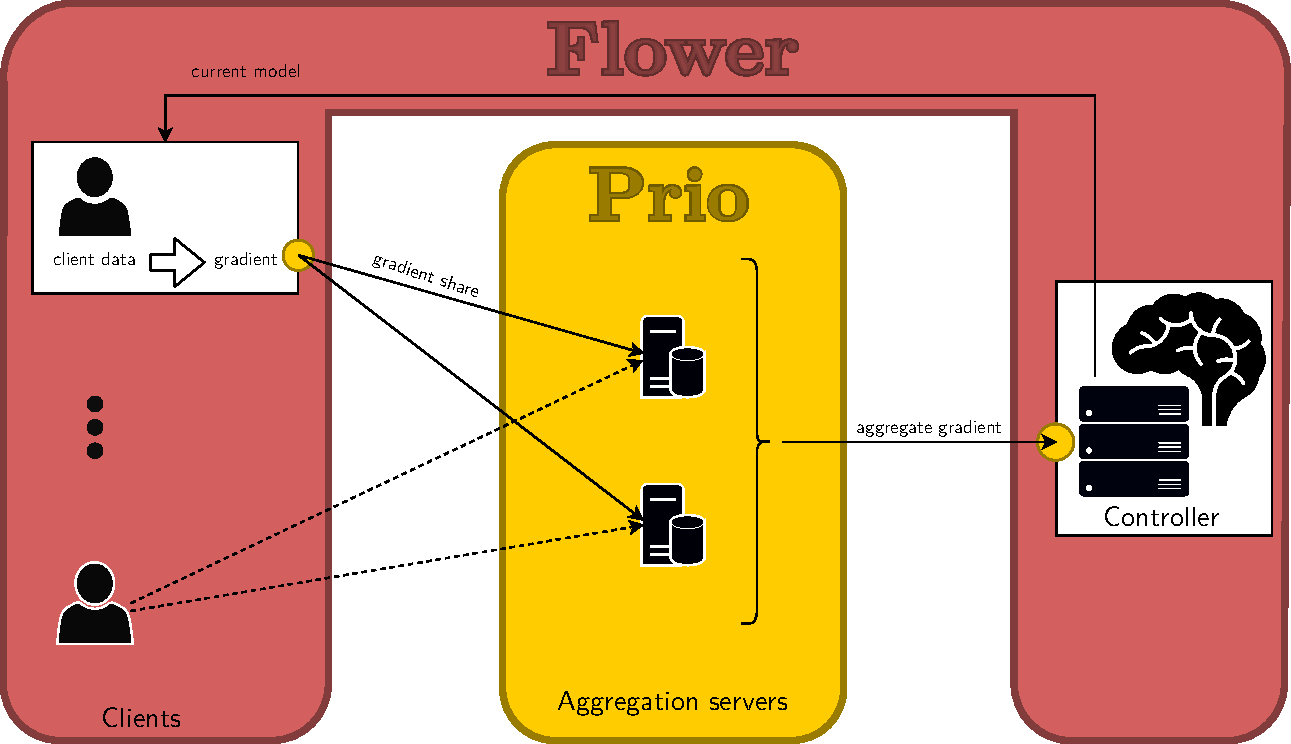
\includegraphics[width=\columnwidth]{assets/dpsa-overview-2-edit_no_explanations-2023-08-22.drawio-edit_rectangle_raw-joined-text_littleproblem-fixed-textfont.pdf}
  \caption{Schematic architecture of an FL system using \texttt{dpsa4flwr}}
  \label{fig:architecture}
\end{figure}

The FL framework remains responsible for all functionality of the training
process, except for gradient aggregation. This includes broadcasting of the
current model, selecting clients for training, and applying the aggregated
gradients to the model.

The aggregation servers execute the Prio protocol, thereby computing the sum of
the clients' gradients, without the need to disclose individual gradients to
anyone. They also verify that all individually submitted vectors have L2-norm
less than one. Finally, before revealing the aggregated gradient to the
controller, each aggregation server adds noise to their own aggregate share, in
order to ensure differential privacy.

The \texttt{dpsa4fl} stack provides the glue code for making this all
work.

\subsection{Integration with an FL framework}
We begin by describing how \texttt{dpsa4fl} is intended to be used by FL
frameworks, using \texttt{flower} as the example target framework.

Before starting the training process, the controller notifies both aggregators
that it's starting a training session with a given id. The aggregators store
session related information under this id. No further \texttt{dpsa4fl}-specific
setup has to be done.
In each round of training, the following sequence of actions happens:
\begin{enumerate}[itemsep=0mm]
\item \texttt{dpsa4fl}: The controller notifies both aggregators that it's
  starting a training round, and receives a task id under which it can collect
  the aggregation result.
\item \texttt{Flower}: The controller selects available clients for this round
  and broadcasts its model as well as the task id to them.
\item \texttt{Flower}: The clients train their copy of the model on their local training data and
  compute the overall gradient vector.
\item \texttt{Flower}: They use flower's aggregation method to notify the
  controller that they have succeeded with training, but don't transmit the gradient.
\item \texttt{dpsa4fl}: They split and encode the gradient vector according to the prio protocol
  and submit each part to an aggregation server under the given task id.
\item \texttt{Prio}: The aggregation servers aggregate reports from all clients, verify them,
  add noise for differential privacy and compute the sum of all gradient vector shares.
\item \texttt{dpsa4fl}: The controller collects the aggregate gradient vector via its task id.
\item \texttt{Flower}: It applies the gradient to the global model, and begins the next round.
\end{enumerate}


\section{Threat model and guarantees}
The controller and the clients have different goals, so their threat models
have to be considered separately. The parties running the aggregation
servers should be impartial to the learning process, but of course might deviate
from that behaviour. We consider the perspectives of the clients
and of the controller below.

\paragraph{Clients.} The clients are interested in participating in an FL-scheme
without their private information becoming known by other parties. There are two
ways this might happen:
\begin{enumerate}
\item The submitted gradient vector of a client (for any training round) might
  become known to other parties. This would allow them to infer properties of
  the clients' local training set.
\item Access to the trained model makes it possible to make inferences about the
  combined training set. Combination with other publicly available data can lead to
  leakage of individual clients' data.
\end{enumerate}
Our system guarantees the following: As long as at least one aggregation server
follows the protocol (i.e., is honest-but-curious), the client's data remains
private.

Attack (1) is mitigated by the secure aggregation mechanism of Prio.
Each aggregation server receives only a share
the clients' gradient vectors. It is impossible to reconstruct the original
vector from this share alone. All processing on the aggregation server, i.e.
the verification, aggregation and noising, happens entirely on its shares.
This means that, as long as the aggregation servers don't collude, they don't
have access to individual gradients.

Attack (2) is mitigated by the fact that the sum of
gradient vectors is never revealed by itself, but only together with the noise added by
both aggregation servers. As long as at least one aggregation server adds
correctly configured noise, this makes the revealed value differentially
private. Differential privacy mitigates inference attacks {\color{red}TODO: source}.

In practice this means: clients can be sure that their data is safe as long as
they trust one of the aggregation servers to be honest in their execution of the
protocol. No trust in the controller is required.

\paragraph{Controller.} The controller is interested in training an ML model on
the data of the clients. Since it cannot inspect the individually submitted
gradients, this introduces the possibility of data poisoning attacks: malicious
clients can try to influence the learning process by submitting exaggerated
gradient vectors.

The input validation capability of Prio mitigates this sort of attack.
As part of the aggregation process, the aggregators verify that each submitted gradient vector
has an L2-norm less than $1$. This means that while clients can still submit
``false'' data, they cannot gain disproportionate leverage by doing so. Prio can only
guarantee this as long as the aggregation servers do not collude with malicious
clients, as in that case it would be easy to craft submissions to fool the other
aggregation server into believing that reports are well-formed, even though they
are not.

In practice this means: the controller can be sure that it receives gradients
based on real data, as long as it trusts \textit{both} aggregation servers to
execute the protocol honestly, and clients do not collude to collectively poison the model.





\section{Privacy analysis}

The protocol describes a distributed implementation of the usual differentially private gradient descent \cite{Abadi_2016}, with the differences being the integer encoding of the gradient vector to enable secret sharing according to the prio protocol \cite{prio}, the aggregation happening on a different machine than the training itself, and the use of discrete Gaussian noise on the integer encoding of the gradient aggregate.
\begin{algorithm}[h]
  \caption{Client procedure}\label{alg:client}

  \begin{algorithmic}[1]
  \Require Training dataset $X$, loss function $\mathcal L(\theta; x)$, number of rounds $N$, fixed-point encoding bit length $b$, set of aggregator server addresses $\texttt{S}$
  \Ensure Model $\theta$ trained on dataset $X$ for $N$ rounds

  \State $\textbf{round}_{(b,0)}(x) = \textbf{sign}(x) \cdot \textbf{floor}_b(|x|)$ \Comment{round to $b$ bits towards zero}
  \State $\pi(x) = 2^{b-1}\cdot (x + 1)$ \Comment{project fixed-point $x\in(-1,1)$ to an integer $\leq 2^b$}

  \For{$N$}\label{lst:line:loop}
  \State$\theta$ = retrieve current shared model from controller\label{lst:line:retrieve}
  \State$\textbf{g}$ = $\frac{1}{|X|} \sum_{x\in X} \nabla\mathcal L(\theta; x)$ \Comment{compute model gradient average}
\label{lst:line:grad}
  \State$\textbf{g}_{clip}$ = $\textbf{g}/\mathbf{max}\{1,||\textbf{g}||_{L_2}\}$ \Comment{clip $\textbf{g}$ to $L_2$ norm 1}\label{lst:line:clip}
  \State$\textbf{g}_{fixed}$ = \Call{\textbf{map}}{$\textbf{round}_{(b,0)}$,$\textbf{g}_{clip}$} \Comment{round to get $b$-bit fixed-point vector}
  \State$\textbf{g}_{int}$ = \Call{\textbf{map}}{$\pi$,$\textbf{g}_{fixed}$} \Comment{project to integer vector}
\label{lst:line:project}
  \State send one secret share of $\textbf{g}_{int}$ to each of the aggregation servers in \texttt S
  \EndFor
  \State$\theta$ = retrieve current shared model from controller
  \State\Return $\theta$
  \end{algorithmic}
\end{algorithm}



\begin{algorithm}[h]
  \caption{Aggregator server procedure}\label{alg:server}
  \begin{algorithmic}[1]
  \Require Set of client addresses $\texttt{C}$, set of aggregator server addresses $\texttt{S}$, privacy parameter $\rho$, fixed-point encoding bit length $b$
  \Ensure Aggregate gradient, noised to be $\rho$-zero-concentrated differentially private

  \State$\textbf{verify}_{\texttt{S}}(\textbf x)$ = perform prio protocol with the other aggregators in \texttt{S} to verify $\textbf x$ is a share of a fixed-point vector with $L_2$ norm $\leq 1$ with entries projected to the integers $\{0,...,2^b\}$ using $\pi$
  \State$\textbf{decrypt}_{\texttt{S}}(\textbf x)$ = perform prio protocol with the other aggregators in \texttt{S} to combine their aggregate shares with $\textbf x$ and obtain the aggregation result
  \State$\textbf{noise}(x) = x+n$ where $n$ is drawn from a discrete Gaussian distribution $\mathcal N_\mathbb{Z}\left(0,\frac{2^{2b}}{2\rho}\right)$
  \State$\pi'(y) = 2^{1-b} \cdot y - |\texttt{C}|$ \Comment{project integer $\leq 2^b\cdot|\texttt{C}|$ to float}
  \State\textbf{G} = 0
  \For{all clients $\texttt{c} \in \texttt{C}$}
       \State{\textbf{g} = retrieve gradient share from \texttt{c}}
	   \State$\textbf{verify}_\texttt{S}(\textbf{g})$ \label{lst:line:verify}
	   \State\textbf{G} = \textbf{G} + \textbf{g}
  \EndFor
  \State$\textbf{G}_{noised} = \textbf{map}(\textbf{noise}, \textbf{G})$  \Comment{add noise componentwise} \label{lst:line:noise}
  \State$\textbf{G}_{agg} = \textbf{decrypt}_{\texttt{S}}(\textbf{G}_{noised})$ \Comment{combine shares to aggregate}
  \State$\textbf{G}_{float} = \textbf{map}(\pi', \textbf{G}_{agg})$ \Comment{map to float vector}
  \State send $\textbf{G}_{float}$ to controller
  \end{algorithmic}
\end{algorithm}

We claim that executing Algorithms 1 and 2 with non-colluding aggregation servers, one of which honestly but curiously follows protocol, and an arbitrary number of potentially malicious clients, provides $(N \cdot \rho)$-zero-concentrated differential privacy for any honest clients' dataset. If both servers are honest, the protocol also protects against data poisoning attacks by malicious clients.

\paragraph{Privacy}
We perform the privacy analysis from the point of view of one client executing one iteration of the loop starting at line~\ref{lst:line:loop} of Algorithm~\ref{alg:client} faithfully. We show that:
\begin{enumerate}
\item The function mapping the clients' dataset to the gradient whose shares are transferred to the aggregation servers is $2^b$-sensitive.
\item No information about the gradient except its secret shares is revealed to any party prior to noising.
\item The noise added on the aggregation server provides $\rho$-zero-concentrated differential privacy for the aggregation result.
\end{enumerate}
It follows that the execution of Algorithm~\ref{alg:client} provides $(N\cdot\rho)$-zero-concentrated differential privacy by the composition property \cite[Lemma~1.8 on page 7]{DBLP:journals/corr/BunS16}.

\begin{enumerate}
\item We want to determine the sensitivity in the dataset $X$ of one iteration of the loop starting at line~\ref{lst:line:loop} of Algorithm~\ref{alg:client}. Assuming the current shared model $\theta$ retrieved in line~\ref{lst:line:retrieve} was computed in a way that provides differential privacy for $X$, its use will not affect the sensitivity. The clipping in line~\ref{lst:line:clip} ensures that 
\[\|\textbf{g}_{fixed}\|_2 = \|\overline{\textbf{round}}_{(b,0)}(\textbf{g}_{clip})\|_2\leq\|\textbf{g}_{clip}\|_2\leq 1.\]
Denote by $\textbf{g}'$ the values of the variables in the algorithm obtained by replacing any one entry in $X$ by a different entry, and by $\overline\pi$ the component-wise application of the function $\pi$. We have
\begin{align*}
\|\textbf g_{int} - \textbf g_{int}'\|_2 &= \|\overline\pi(\textbf g_{fixed}) - \overline \pi(\textbf g_{fixed}')\|_2 \\
&\leq 2^{b-1} \cdot \| \textbf g_{fixed}- \textbf g_{fixed}'\|_2\\
&\leq 2^{b-1} \cdot (\| \textbf g_{fixed}\|_2 + \|\textbf g_{fixed}'\|_2)\\
&\leq 2^b
\end{align*}
One iteration of the computation inside the loop (lines~\ref{lst:line:retrieve} to \ref{lst:line:project}) therefore is $2^b$-sensitive in $X$.

\item Prio secret sharing amounts to the client splitting their secret into summands, and recovering the aggregated shares amounts to summing the sums of secret shares \cite[Scheme on page 3]{prio}. Doing so does not affect the sensitivity of $\textbf{g}_{int}$, as the result of the computation is equal to the result obtained by summing all clients' gradients without secret sharing. Share transfer happens over an encrypted channel \cite[Step 1 of Scheme on page 3]{prio}, combining the shares happens after adding noise on the server in line~\ref{lst:line:noise}. Therefore if at least one of the servers is honest and they don't collude, the only things visible to anyone eavesdropping or participating are single secret shares of the gradient and the noised aggregate.

\item Noise is added prior to combining the aggregate shares to avoid disclosing the non-noised aggregate to a server. Since combining them simply means computing their sum \cite[Step 3 of Scheme on page 3]{prio}, the value of $\textbf{G}_{agg}$ does not depend on whether the noise is added before or after combining the shares. We can hence view the function mapping one clients' data set $X$ to the non-noised gradient aggregate as a $2^b$-sensitive function over the integers, so adding noise drawn from $\mathcal N_\mathbb{Z}\left(0,\frac{2^{2b}}{2\rho}\right)$ will provide $\rho$-zero-concentrated differential privacy due to~\cite[Theorem 14 on page 15, with all $\sigma_j=\frac{2^{2b}}{2\rho}$]{DBLP:journals/corr/abs-2004-00010}. Mapping the integer encoding of the aggregate back to a float vector and using it in further training will not affect privacy due to post-processing invariance. Note that each server adds the entire amount of noise required to obtain the guarantee, so if at least one of them is honest the guarantee holds. This comes at the cost of adding the entire noise on each server, resulting in worse utility.
\end{enumerate}

\paragraph{Robustness}
In line~\ref{lst:line:verify} of Algorithm~\ref{alg:server}, the servers perform a secret-shared non-interactive proof protocol \cite[Section 4]{prio} together to verify that the client-side clipping was performed properly. This ensures the sensitivity is as described above, even for gradients submitted by malicious clients, and hence protects from clients attempting to influence the computation result disproportionately. The verification part of the protocol requires all servers to act honestly, so our system offers this protection only under a weaker threat model. The above proof of privacy still holds for all clients that execute the protocol truthfully.

\section{Evaluation}

\subsection{Utility analysis}
We want to know how much noise our algorithm adds compared to the standard gradient descent with differential privacy obtained by sampling from the regular normal distribution~\cite{Abadi_2016}. There, each iteration of gradient aggregation adds noise drawn from $\mathcal N\left(0,\frac{(2C)^2}{2\rho}\right)$ for gradients clipped to norm $C$ ($C=1$, in our case) and our notion of $\rho$-zero-concentrated differential privacy.

Consider rounding both gradient entries and noise to obtain $b$-bit fixed point numbers with one integer bit. Rounding a gradient introduces an error
$$|\textbf{round}_{0,b)}(x) - x|\leq\frac{1}{2^{b-1}}$$
to each of the clients' gradient entries in each aggregation step. This should be negligible given that the noise added to each aggregate entry is sampled from a normal distribution with standard deviation of $\sqrt{\frac{2}{\rho}}$, meaning that even for large values of $\rho$, say $\rho = 2^6$, and small values of $b$, say $b=16$, still $99.88\%$ of the noise samples will be an order of magnitude larger than that error.

Next consider applying the projection $\pi$ to both gradients and noise before applying the noise, and reversing the projection afterwards. This does not alter the magnitude of the noise in the end result, and is equivalent to sampling instead from a scaled rounded Gaussian distribution $\mathcal N_{round}\left(0,\frac{2^{2b}}{2\rho}\right)$.

Next consider using the discrete Gaussian instead. \cite[Corollary 17]{DBLP:journals/corr/abs-2004-00010} shows that utility is strictly better by a small amount.

Last, consider that our protocol simply is a modification of the regular gradient descent algorithm with differential privacy as described in this section, but the aggreagtion and addition of noise is distributed among multiple servers $\texttt{S}$. As described in our threat model, in order to require trust in only one of those servers, each server has to add the entire amount of noise, so noise magnitude worsens by a multiple of $|\texttt{S}|$. The sum of discrete Gaussian variables is distributed closely Gaussian~\cite[Theorem 11]{Kairouz2021TheDD}, so utility of our algorithm with $\rho$-ZCdp is approximately that of the regular gradient descent with $|\texttt{S}|\cdot\rho$-ZCdp. If all aggregators are trustworthy, the protocol can be adapted so each only adds a fraction of the total noise to improve utility while maintaining the privacy bound.


\subsection{Communication complexity}
The communication costs of transmitting the clients' gradients in a
differentially private way compared to transmitting plaintext data is an
important metric for evaluating aggregation protocols for FL. Since gradients
are typically large (e.g. [TODO: insert size here]), their transmission accounts
for most of the time complexity of the whole learning procedure.

In the prio protocol, the message size is mostly determined by the size of the
encoded gradient together with the size of the encoded proof of its
well-formedness. Two such messages must be sent per aggregation, one to each
aggregator. Other messages sent as part of the prio protocol are negligible.

In our current implementation of \texttt{dpsa4fl} we use a naive encoding of
gradient entries as field elements. This results in a rather large blow-up of
message size. Currently, a single 16-bit fixed point number is encoded by 16
128-bit field elements, which means that our messages are at least 128 times
the size of plaintext gradients.
There are both trivial and more complex methods to improve on this: the field
size of 128-bit can be reduced to 64-bit while still supporting gradients with
up to $2^{34} \approx 17 \cdot 10^9$ entries. Furthermore, the encoding can be
compactified, such as not to require a seperate field element for each
transmitted bit. Since this will increase the size of the correctness proof,
a balance which optimizes message size has to be found.


{\color{green}TODO: maybe give some context to the image?}
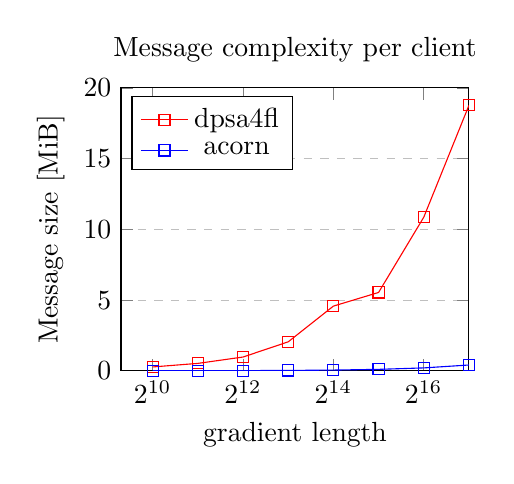
\begin{tikzpicture}
  \begin{axis}[
    title={Message complexity per client},
    xlabel={gradient length},
    ylabel={Message size [MiB]},
    xmode=log,
    log basis x=2,
    xlabel=gradient length,
    ymode=normal,
    % ymode=log,
    % log ticks with fixed point,
    xmin=0, xmax=2^17,
    ymin=0, ymax=20,
    % xtick={0,20,40,60,80,100},
    % ytick={0,20,40,60,80,100,120},
    legend pos=north west,
    ymajorgrids=true,
    grid style=dashed,
    ]

    \addplot[
    color=red,
    mark=square,
    ]
    coordinates {
      (2^10,0.2738359375)(2^11,0.525400390625)(2^12,0.97528125)(2^13,2.049)(2^14,4.574)(2^15,5.539)(2^16,10.855)(2^17,18.761)
    };
    \addlegendentry{dpsa4fl}

    \addplot[
    color=blue,
    mark=square,
    ]
    coordinates {
      (2^10,0.0044921875)(2^11,0.00771484375)(2^12,0.0142578125)(2^13,0.02705078125)(2^14,0.052734375)(2^15,0.10400390625)(2^16,0.2064453125)(2^17,0.411328125)
    };
    \addlegendentry{acorn}
  \end{axis}
\end{tikzpicture}

\section{Conclusion}
While the previous section concerning message complexity
illustrates that \texttt{dpsa4fl} is not yet ready for real-world deployment, the
existing work is quite promising. The \texttt{libprio-rs} and \texttt{janus}
libraries were comparably easy to extend, and the threat model provided by Prio
seems to be strong and yet pragmatic enough for it to gain widespread adoption.
Ideas for approaches to minimize message sizes exist, and are left for future work.

\bibliographystyle{plainnat}
\bibliography{doc}

\end{document}

